\chapter{Resultados y discusión}

En este capítulo se presentan y analizan los resultados obtenidos tras aplicar el flujo completo del sistema. En primer lugar se estudia la separabilidad del espacio de características, para entender cómo se organizan los datos antes de evaluar los modelos. A continuación se comparan los resultados de entrenamiento y se interpretan las salidas de explicabilidad, relacionando las métricas obtenidas con las decisiones tomadas durante el desarrollo.

\section{Análisis de separabilidad}


Antes de entrenar los modelos, se estudió la separabilidad del espacio de características para observar cómo se organizaban los datos. El objetivo de este análisis es comprobar si las muestras tienden a agruparse de forma natural según la emoción presentada o si, por el contrario, la variabilidad entre sujetos domina la distribución. Esta revisión permite orientar e interpretar mejor la comparación posterior entre el entrenamiento \textit{all-subjects} y el entrenamiento \textit{within-subject}.


\subsection{Interpretación de las representaciones}

Para interpretar esta sección conviene recordar brevemente el flujo seguido por el análisis. El programa parte de la matriz de características ya generada y utiliza el mismo conjunto de variables que después se emplea en los clasificadores: potencia Alpha, potencia Beta y asimetría Alpha, características habituales en estudios de reconocimiento emocional con \ac{EEG} \cite{alarcao2019eeg,smith2017frontal}. A partir de ese espacio, genera proyecciones bidimensionales con \ac{PCA} y \ac{LDA}, tanto con todas las épocas juntas como separando el análisis por sujeto.

La idea no es entrenar todavía un clasificador, sino observar la forma del espacio de datos. Por eso, las figuras se colorean de dos maneras: por condición emocional y por sujeto. Si los puntos se agrupan mejor por emoción, el problema sería más favorable para un modelo común; si se agrupan mejor por participante, la variabilidad intersujeto puede dificultar el entrenamiento \textit{all-subjects}, un problema habitual en clasificación de señales \ac{EEG} entre participantes \cite{lotte2007classification,rajpoot2022subject}.

En las figuras de \ac{PCA}, cada punto representa una época proyectada en dos dimensiones. La técnica no selecciona unas épocas concretas, sino que usa todas las muestras para calcular nuevos ejes de representación. Estos ejes no corresponden a canales ni bandas concretas, sino a combinaciones lineales de características orientadas a conservar la mayor varianza posible del conjunto \cite{sklearnPcaDocs}. Por eso, esta representación resulta útil para observar la estructura natural de los datos: si los puntos se agrupan por sujeto, significa que esa fuente de variación pesa más que la separación emocional.


El porcentaje que aparece junto a cada eje, como \texttt{PC1 50\%}, indica cuánta variabilidad de los datos originales queda resumida en esa dirección. No representa exactitud del modelo: si \texttt{PC1} y \texttt{PC2} suman, por ejemplo, un 70\%, la figura conserva aproximadamente ese porcentaje de la estructura total del conjunto.

En las figuras de \ac{LDA} también se proyectan todas las épocas, pero los ejes se calculan con un criterio distinto: se utilizan las etiquetas de emoción para buscar direcciones discriminativas entre \texttt{JOY}, \texttt{NEUTRO} y \texttt{SAD} \cite{sklearnLdaDocs}. Por este motivo suele verse una separación más clara que en \ac{PCA}: la figura no muestra únicamente dónde varían más los datos, sino el plano donde las clases quedan más diferenciadas. Aun así, estas representaciones deben entenderse como una ayuda visual para estudiar la estructura del conjunto, no como una medida final de rendimiento del clasificador.


Por tanto, si la separación entre emociones es menor en \ac{PCA} que en \ac{LDA}, no significa necesariamente que las características no contengan información emocional. Más bien sugiere que, al analizar todos los participantes en un espacio común, la variabilidad propia de cada sujeto condiciona la estructura del espacio de características y puede enmascarar parcialmente la separación entre condiciones emocionales. La \ac{LDA} puede mostrar una separación más clara porque busca explícitamente las direcciones que maximizan la diferencia entre clases, mientras que la \ac{PCA} puede reflejar otros factores dominantes, como las diferencias individuales entre participantes.

Por último, para apoyar esta lectura visual se utilizaron dos métricas. El \textit{ratio} centroides/dispersión compara la distancia media entre los centros de los grupos con la dispersión interna de esos mismos grupos. El centroide puede entenderse como el punto medio de todas las épocas de una emoción o de un sujeto, mientras que la dispersión indica cuánto se alejan las épocas de su propio centro. Por tanto, un valor bajo significa que los grupos están muy solapados o poco separados respecto a su tamaño, mientras que un valor alto indica grupos más compactos y alejados entre sí. La \textit{silhouette} resume una idea similar: mide si cada época queda más cerca de su propio grupo que de los demás \cite{rousseeuw1987silhouettes}. Valores cercanos a cero indican solapamiento, valores positivos indican mejor separación y valores negativos sugieren que algunas muestras encajan peor en el grupo asignado.

\subsection{Separabilidad global}

La primera comprobación consistió en representar todas las épocas en un único espacio común, equivalente al escenario \textit{all-subjects}. En este análisis, la normalización se ajusta de forma global; la referencia \texttt{NEUTRO} se calcula con todas las épocas neutras disponibles, agregando todos los participantes. Por tanto, cuando una figura aparece coloreada por sujeto, no se está recalculando un espacio distinto para cada participante; se muestran las mismas coordenadas globales, pero cambiando el color para comprobar si la estructura se organiza mejor por emoción o por sujeto.

\begin{figure}[H]
    \centering
    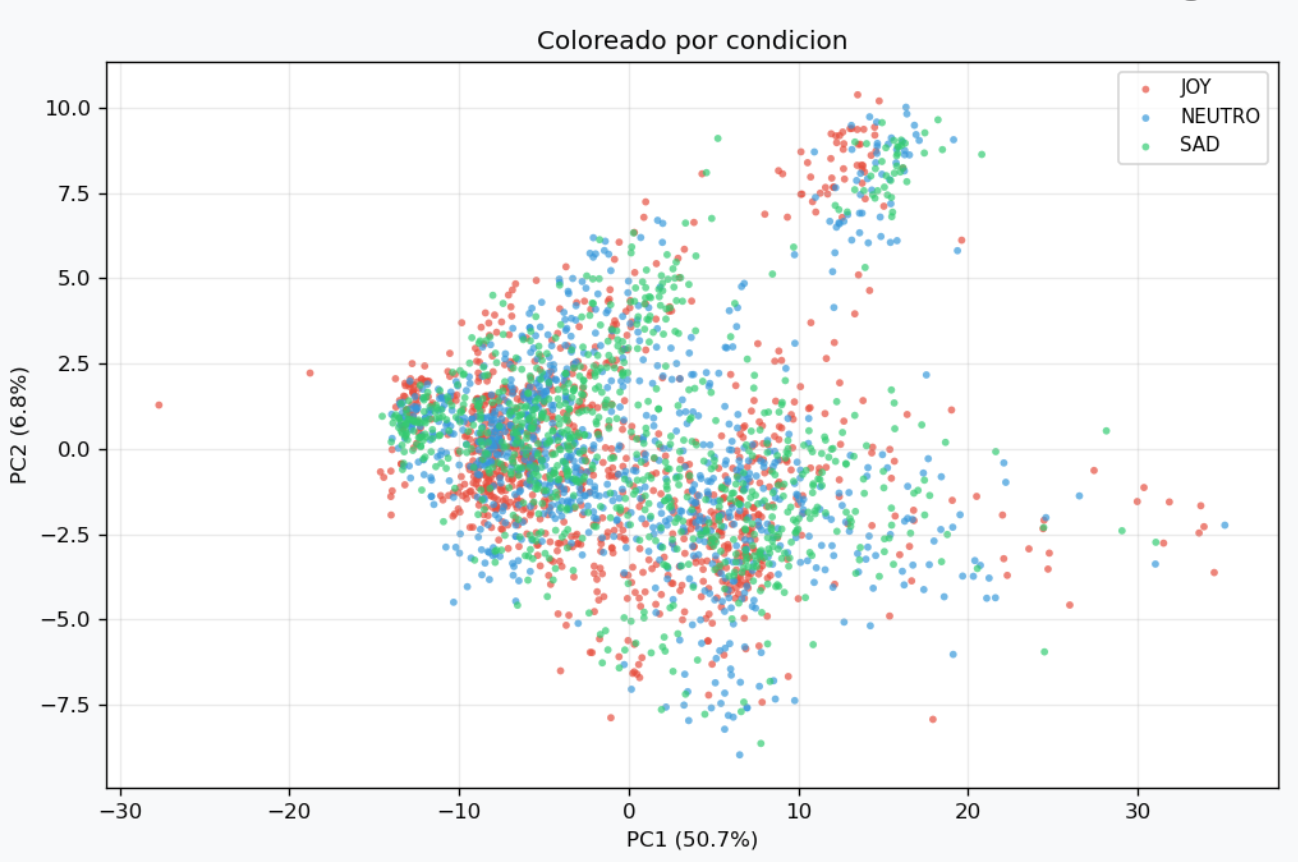
\includegraphics[width=0.78\textwidth]{figs/separability/PCA_global_condicion.png}
    \caption{\ac{PCA} global del espacio de características coloreada por condición emocional.}
    \label{fig:pca_global_condicion}
\end{figure}

En la Figura~\ref{fig:pca_global_condicion}, la proyección \ac{PCA} coloreada por condición muestra una mezcla considerable entre \texttt{JOY}, \texttt{NEUTRO} y \texttt{SAD}. Aunque existen zonas con mayor densidad de algunas clases, no aparecen grupos emocionales claramente separados. Esto indica que las direcciones de máxima varianza del conjunto no están dominadas principalmente por la condición emocional.


\begin{figure}[H]
    \centering
    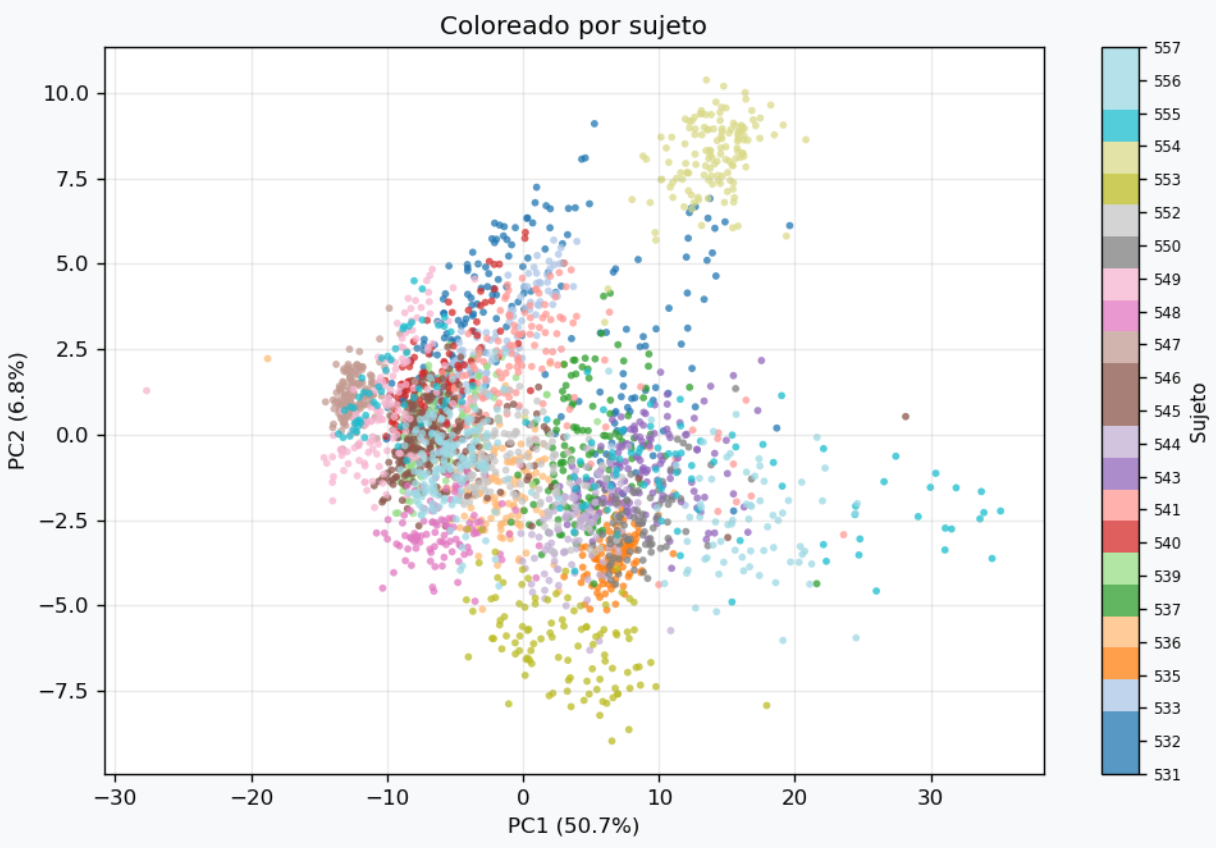
\includegraphics[width=0.78\textwidth]{figs/separability/PCA_global_sujeto.png}
    \caption{\ac{PCA} global del espacio de características coloreada por sujeto.}
    \label{fig:pca_global_sujeto}
\end{figure}

La misma proyección, coloreada por participante, se muestra en la Figura~\ref{fig:pca_global_sujeto}. En este caso se aprecia una organización más marcada: varias regiones del plano concentran épocas de sujetos concretos. Esta comparación sugiere que una parte importante de la variabilidad recogida por la \ac{PCA} está relacionada con diferencias individuales entre participantes, más que con la separación directa entre las tres emociones, algo coherente con la dificultad descrita en modelos independientes del sujeto \cite{rajpoot2022subject}.




\begin{figure}[H]
    \centering
    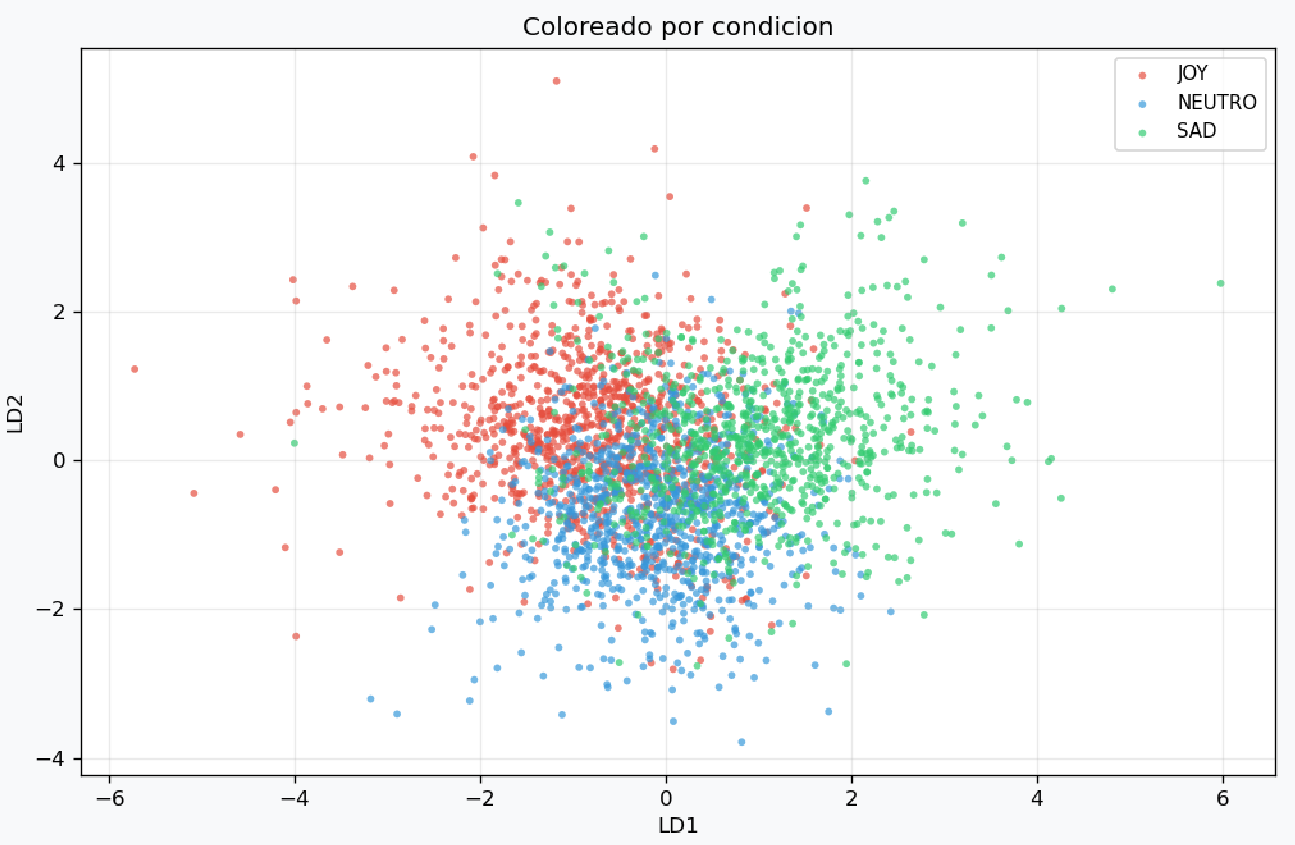
\includegraphics[width=0.78\textwidth]{figs/separability/LDA_global_condicion.png}
    \caption{\ac{LDA} global del espacio de características coloreada por condición emocional.}
    \label{fig:lda_global_condicion}
\end{figure}

En la Figura~\ref{fig:lda_global_condicion} se observa una separación más clara que en \ac{PCA}: \texttt{JOY} tiende a desplazarse hacia una zona del plano, \texttt{SAD} hacia otra y \texttt{NEUTRO} queda en una región intermedia con solapamiento. Esta mejora visual indica que las características contienen información útil para discriminar emociones, aunque la separación no sea perfecta.



\begin{figure}[H]
    \centering
    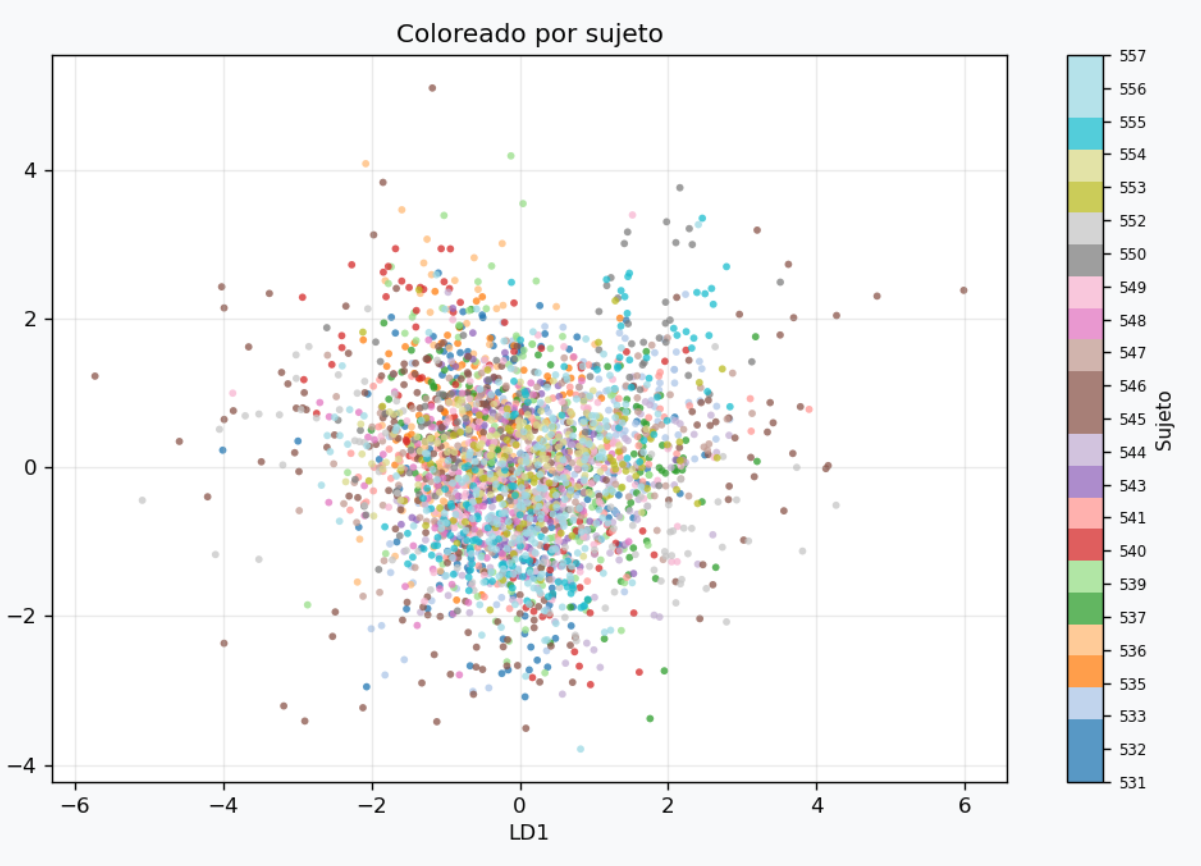
\includegraphics[width=0.78\textwidth]{figs/separability/LDA_global_sujeto.png}
    \caption{\ac{LDA} global del espacio de características coloreada por sujeto.}
    \label{fig:lda_global_sujeto}
\end{figure}

La Figura~\ref{fig:lda_global_sujeto} utiliza las mismas coordenadas \ac{LDA}, pero coloreadas por sujeto. En este caso los colores aparecen más mezclados que en la \ac{PCA} coloreada por sujeto, porque la proyección está orientada a separar emociones y no participantes. Aun así, la dispersión sigue siendo elevada, lo que refuerza la idea de que el análisis global contiene información emocional, pero continúa afectado por la variabilidad intersujeto.


En el espacio original, el ratio centroides/dispersión para las emociones es 0,10 y la \textit{silhouette} es prácticamente nula, por lo que las tres condiciones aparecen muy mezcladas. Sin embargo, al usar el sujeto como etiqueta, el ratio aumenta hasta 2,46, lo que indica que las épocas se agrupan mejor por participante que por emoción. En \ac{PCA} ocurre algo similar: la separación por emoción sigue siendo baja, mientras que la organización por sujeto resulta más evidente. En \ac{LDA}, al usar las etiquetas emocionales para construir la proyección, el ratio por condición aumenta hasta 1,34. Por tanto, el espacio global no carece de información emocional, pero esta queda diluida cuando se mezclan todos los participantes en una única representación.

\subsection{Separabilidad dentro de cada sujeto}

Al repetir el análisis de forma individual, la referencia \texttt{NEUTRO} se calcula con las épocas neutras del propio participante. De esta forma, cada sujeto se compara consigo mismo y no contra una media global formada por todos los registros.

Las Figuras~\ref{fig:pca_within_547_552} y~\ref{fig:lda_within_547_552} muestran dos ejemplos representativos: los sujetos 211-000547 y 211-000552. Se han elegido los mismos participantes para \ac{PCA} y \ac{LDA} con el objetivo de observar cómo cambia la estructura cuando se analiza cada registro dentro de su propio contexto.

\begin{figure}[H]
    \centering
    \begin{minipage}{0.48\textwidth}
        \centering
        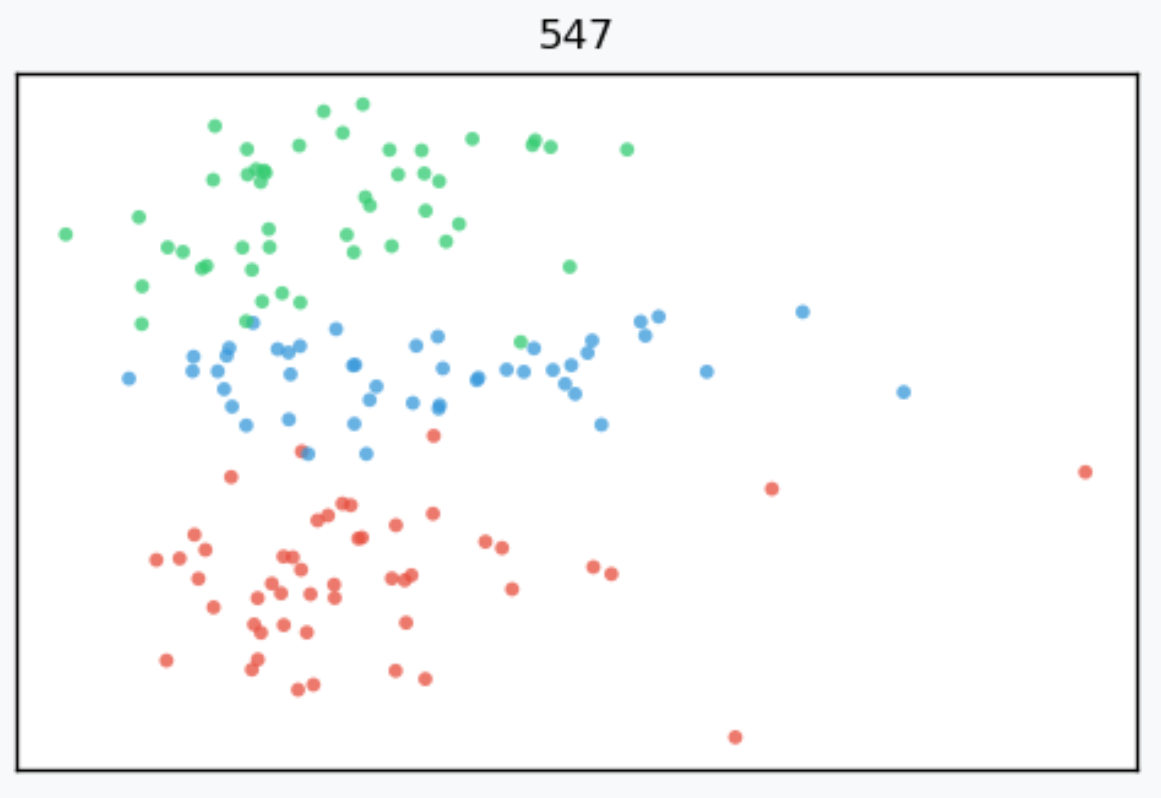
\includegraphics[width=\textwidth]{figs/separability/pca_547.png}

        \small Sujeto 211-000547
    \end{minipage}
    \hfill
    \begin{minipage}{0.48\textwidth}
        \centering
        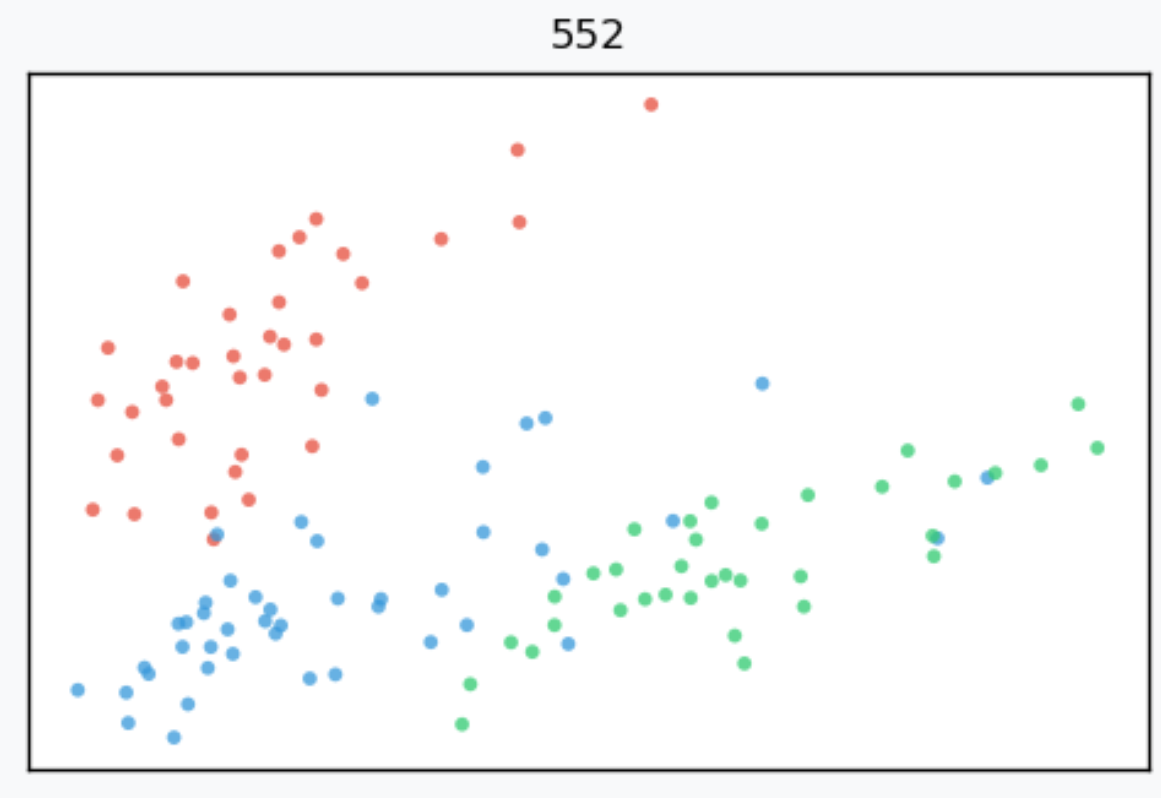
\includegraphics[width=\textwidth]{figs/separability/pca_552.png}

        \small Sujeto 211-000552
    \end{minipage}
    \caption{\ac{PCA} dentro de sujeto para dos participantes.}
    \label{fig:pca_within_547_552}
\end{figure}

En la Figura~\ref{fig:pca_within_547_552} las emociones aparecen más organizadas que en la proyección global, aunque la separación no es idéntica en los dos casos. En el sujeto 211-000547 las condiciones muestran cierto solapamiento, mientras que en el 211-000552 los grupos quedan más definidos. Esta diferencia es esperable: cada participante puede presentar una respuesta fisiológica distinta ante los estímulos \cite{alarcao2019eeg,rajpoot2022subject}, y la \ac{PCA} solo muestra las direcciones de mayor variabilidad, no necesariamente las que mejor separan las emociones. Aun así, los valores de separabilidad aumentan respecto al análisis global por emoción: el \textit{ratio} centroides/dispersión pasa de 0,09 en la \ac{PCA} global a 1,77 en el sujeto 211-000547 y a 2,52 en el sujeto 211-000552.

\begin{figure}[H]
    \centering
    \begin{minipage}{0.48\textwidth}
        \centering
        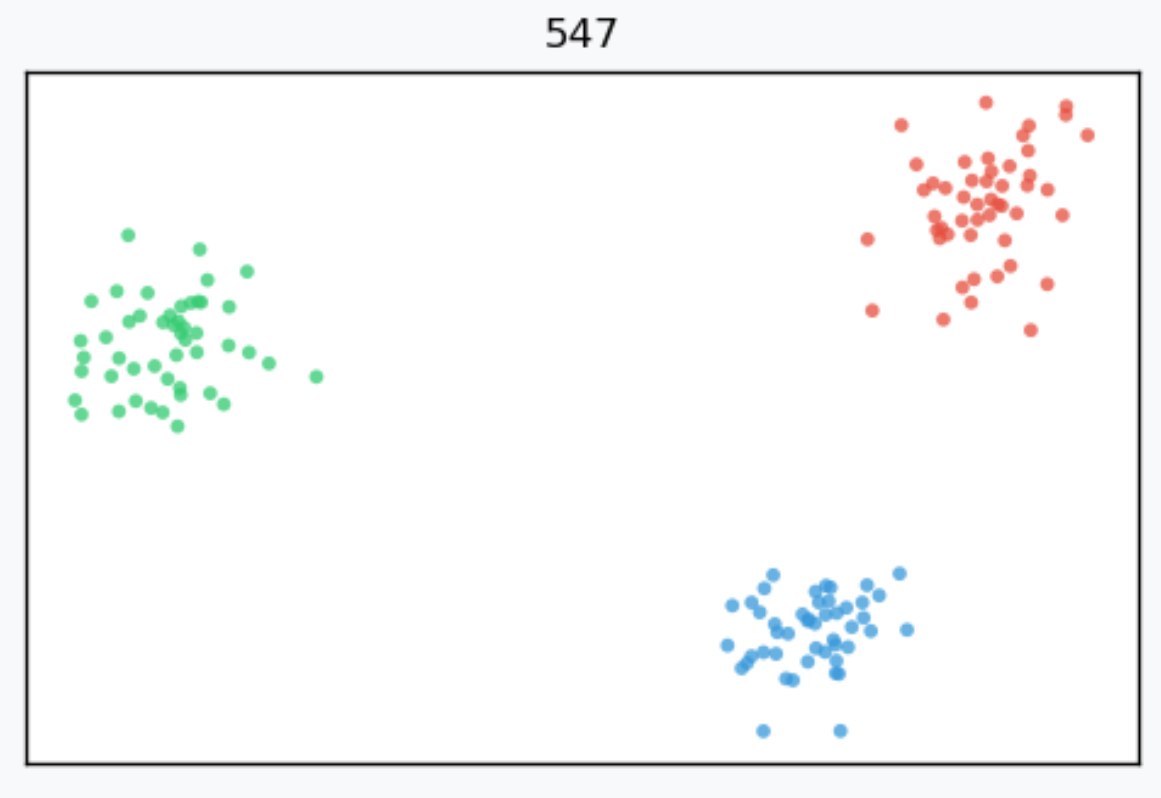
\includegraphics[width=\textwidth]{figs/separability/lda_547.png}

        \small Sujeto 211-000547
    \end{minipage}
    \hfill
    \begin{minipage}{0.48\textwidth}
        \centering
        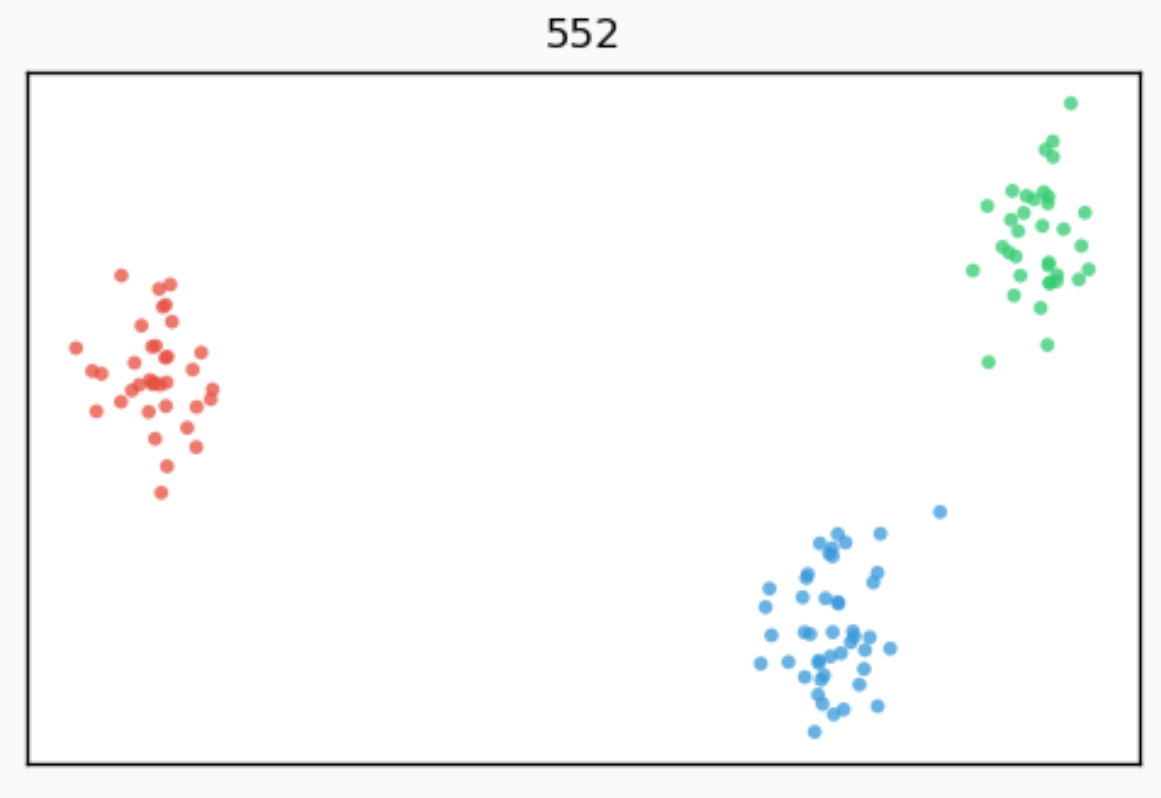
\includegraphics[width=\textwidth]{figs/separability/lda_552.png}

        \small Sujeto 211-000552
    \end{minipage}
    \caption{\ac{LDA} dentro de sujeto para dos participantes.}
    \label{fig:lda_within_547_552}
\end{figure}

La Figura~\ref{fig:lda_within_547_552} muestra una separación mucho más clara entre \texttt{JOY}, \texttt{NEUTRO} y \texttt{SAD}. De nuevo, los dos sujetos no tienen exactamente la misma geometría: las clases se distribuyen con formas y distancias diferentes, lo que confirma que la estructura emocional no se manifiesta igual en todos los participantes. Sin embargo, en ambos casos la separación es claramente superior a la observada al mezclar todos los sujetos. Esto también se refleja en las métricas: el \textit{ratio} centroides/dispersión alcanza 11,24 para el sujeto 211-000547 y 14,68 para el 211-000552, con valores de \textit{silhouette} cercanos a 0,84 en ambos casos.

\subsection{Resumen de separabilidad}

El análisis de separabilidad muestra una tendencia clara: al representar todos los participantes en un mismo espacio, las diferencias individuales tienen un peso muy alto y la separación entre emociones pierde claridad. En cambio, al analizar cada sujeto con su propia referencia neutra, las condiciones emocionales aparecen más organizadas y las métricas de separación aumentan. Por ello, antes de observar las métricas de clasificación, ya se espera que los modelos \textit{within-subject} obtengan una precisión mayor que los modelos \textit{all-subjects}.


\section{Resultados de entrenamiento y evaluación}

Una vez estudiada la separabilidad del espacio de características, se evaluaron los dos clasificadores utilizados en el sistema: regresión logística y árbol de decisión. En ambos casos se empleó el mismo conjunto de entrada, que en el programa anterior. La evaluación se realizó en dos escenarios: \textit{all-subjects}, donde se entrena un modelo común separando los sujetos entre folds, y \textit{within-subject}, donde cada participante se evalúa de forma independiente.

Las métricas principales fueron la exactitud y el \textit{F1-score} macro, calculadas a partir de las predicciones de validación cruzada \cite{sklearnMetrics}. En las matrices de confusión, las filas representan la emoción real y las columnas la emoción predicha. La matriz normalizada permite leer porcentajes por clase; por ejemplo, un valor de 0,96 en la celda \texttt{JOY}-\texttt{JOY} significa que el 96\% de las épocas reales de \texttt{JOY} fueron clasificadas correctamente como \texttt{JOY}.

\subsection{Regresión logística}

En el escenario \textit{all-subjects}, la regresión logística obtuvo una exactitud media de 0,346 y un \textit{F1-score} macro de 0,324. Estos valores están muy próximos al azar para un problema de tres clases, donde una clasificación aleatoria equilibrada estaría alrededor de 0,33. La matriz global muestra además un sesgo claro hacia la clase \texttt{SAD}: muchas épocas reales de \texttt{JOY} y \texttt{NEUTRO} terminan clasificándose como \texttt{SAD}. Esto indica que el modelo común no consigue separar de forma consistente las emociones cuando debe generalizar a sujetos no vistos.

\begin{figure}[H]
    \centering
    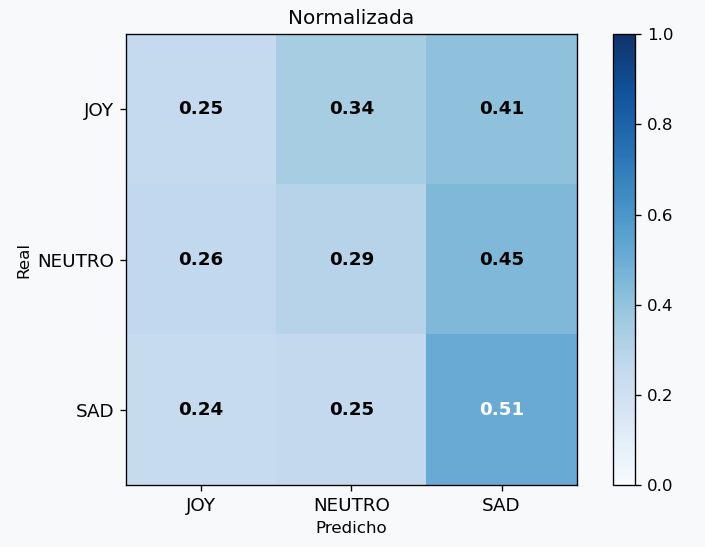
\includegraphics[width=0.68\textwidth]{figs/training/all_subjects/log_reg.png}
    \caption{Matriz de confusión de la regresión logística en el escenario \textit{all-subjects}.}
    \label{fig:confusion_logreg_all}
\end{figure}

La Figura~\ref{fig:confusion_logreg_all} refleja este comportamiento: la diagonal principal no domina la matriz y la última columna concentra muchas predicciones. En concreto, solo el 25\% de las épocas reales de \texttt{JOY} y el 29\% de las de \texttt{NEUTRO} se clasifican correctamente, mientras que \texttt{SAD} alcanza un 51\%. Por tanto, el modelo no aprende una frontera estable entre emociones cuando se evalúa sobre sujetos distintos a los usados en entrenamiento.

\begin{figure}[H]
    \centering
    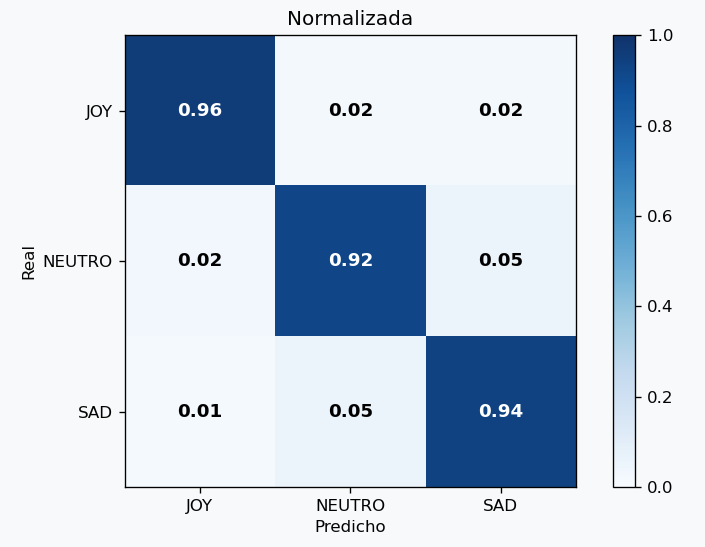
\includegraphics[width=0.68\textwidth]{figs/training/within/logreg.png}
    \caption{Matriz de confusión de la regresión logística en el escenario \textit{within-subject}.}
    \label{fig:confusion_logreg_within}
\end{figure}

La situación cambia claramente en el escenario \textit{within-subject}. La exactitud media por sujeto aumenta hasta 0,944, con un \textit{F1-score} macro de 0,940. En la matriz agregada de la Figura~\ref{fig:confusion_logreg_within}, la diagonal principal concentra la mayor parte de las predicciones: \texttt{JOY} alcanza un 0,96 de acierto por clase, \texttt{NEUTRO} un 0,92 y \texttt{SAD} un 0,94. Aunque todavía existe cierta confusión entre \texttt{NEUTRO} y \texttt{SAD}, los errores son mucho menores que en el modelo global.

También se observa una estabilidad elevada entre participantes, aunque no uniforme. Algunos sujetos alcanzan valores perfectos de exactitud media, mientras que otros se sitúan alrededor de 0,80. Esta variabilidad no invalida el resultado, pero sí confirma que el reconocimiento emocional con \ac{EEG} sigue dependiendo mucho del sujeto analizado. Para consultar todos los resultados de cada modelo en este escenario, puede revisarse el archivo \path{results/within_subject/within_subject_results.json}, disponible en el repositorio del proyecto indicado en el Anexo~\ref{anexo:repositorio}.

\subsection{Árbol de decisión}

El árbol de decisión fue el mejor clasificador en el escenario \textit{all-subjects}, aunque la mejora respecto a la regresión logística fue pequeña. Obtuvo una exactitud media de 0,358 y un \textit{F1-score} macro de 0,346. La matriz de confusión muestra una distribución algo más equilibrada que la de la regresión logística, sin un sesgo tan fuerte hacia una única clase, pero la diagonal sigue siendo débil: los aciertos por clase se mantienen entre 0,33 y 0,39. Por tanto, aunque este clasificador sea ligeramente superior en el modelo común, el rendimiento continúa siendo bajo.

\begin{figure}[H]
    \centering
    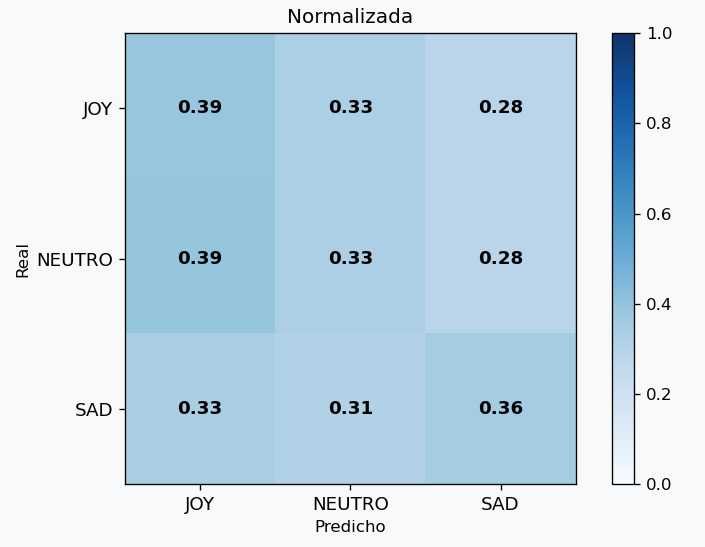
\includegraphics[width=0.68\textwidth]{figs/training/all_subjects/decission_tree.png}
    \caption{Matriz de confusión del árbol de decisión en el escenario \textit{all-subjects}.}
    \label{fig:confusion_tree_all}
\end{figure}

En el escenario \textit{within-subject}, el árbol de decisión obtuvo una exactitud media de 0,851 y un \textit{F1-score} macro de 0,842. La mejora respecto al modelo global es clara, aunque queda por debajo de la regresión logística. En la Figura~\ref{fig:confusion_tree_within}, la clase \texttt{JOY} es la más reconocible, con un 0,88 de acierto por clase. \texttt{NEUTRO} y \texttt{SAD} presentan valores similares, 0,82 y 0,83 respectivamente, con una confusión algo mayor entre ambas condiciones.

\begin{figure}[H]
    \centering
    
\includegraphics[width=0.68\textwidth]{figs/training/within/decission_tree.png}
    \caption{Matriz de confusión del árbol de decisión en el escenario \textit{within-subject}.}
    \label{fig:confusion_tree_within}
\end{figure}



\subsection{Comparación general}

Los resultados confirman la tendencia observada en el análisis de separabilidad. El entrenamiento \textit{all-subjects} no consigue aprender un patrón emocional suficientemente general entre participantes: tanto la exactitud como el \textit{F1-score} macro se mantienen cerca del azar, y las matrices muestran una confusión elevada entre las tres emociones. En cambio, el entrenamiento \textit{within-subject} obtiene resultados claramente superiores, especialmente con regresión logística.

\begin{table}[H]
\centering
\begingroup
\setlength{\tabcolsep}{4.5pt}
\renewcommand{\arraystretch}{1.18}
\begin{tabular}{llccccc}
\hline
\textbf{Clasificador} & \textbf{Escenario} & \textbf{Acc.} & \textbf{F1 macro} & \textbf{JOY} & \textbf{NEUTRO} & \textbf{SAD} \\
\hline
Reg. logística & \textit{all-subjects} & 0,346 & 0,324 & 25\% & 29\% & 51\% \\
Reg. logística & \textit{within-subject} & \textbf{0,944} & \textbf{0,940} & \textbf{96\%} & \textbf{92\%} & \textbf{94\%} \\
Árbol de decisión & \textit{all-subjects} & 0,358 & 0,346 & 39\% & 33\% & 36\% \\
Árbol de decisión & \textit{within-subject} & \textbf{0,851} & \textbf{0,842} & \textbf{88\%} & \textbf{82\%} & \textbf{83\%} \\
\hline
\end{tabular}
\endgroup
\caption{Resumen comparativo de rendimiento por clasificador y escenario. En las columnas de cada emoción se muestra el porcentaje de acierto de esa clase.}
\label{tab:comparacion_entrenamiento}
\end{table}

La diferencia entre ambos escenarios sugiere que las características extraídas son útiles para distinguir emociones dentro de un mismo participante, pero no se trasladan de forma directa entre sujetos. Por ello, el modelo más adecuado para este conjunto de datos es la regresión logística \textit{within-subject}, ya que combina el mayor rendimiento medio con una matriz de confusión más concentrada en la diagonal principal.

\section{Análisis de explicabilidad}

Una vez seleccionado el escenario \textit{within-subject} con regresión logística, se analizaron las explicaciones generadas mediante \ac{SHAP} \cite{lundberg2017shap}. El objetivo de esta sección no es volver a evaluar el modelo, sino observar qué características utiliza con mayor peso para diferenciar \texttt{JOY}, \texttt{NEUTRO} y \texttt{SAD}. Estas explicaciones deben interpretarse como patrones aprendidos por el clasificador a partir de las características disponibles, no como una prueba neurofisiológica directa.

La lectura de estos resultados se contrastó durante el desarrollo con la orientación del tutor y con una revisión cualitativa desde el ámbito médico. Esta comprobación no se plantea como validación clínica, sino como apoyo para interpretar los mapas de forma prudente: primero se describe qué devuelve el modelo y después se valora si la distribución espacial y espectral resulta razonable para una tarea de escucha emocional.

La interpretación se centra en las bandas Alpha y Beta, que fueron las utilizadas en el entrenamiento final. Esta elección es coherente con el contexto experimental y con el uso habitual de características espectrales en reconocimiento emocional con \ac{EEG} \cite{alarcao2019eeg,koelstra2012deap}. Los participantes escuchaban estímulos auditivos en reposo, por lo que se buscó un espacio de características más conservador y menos expuesto a bandas que podían aportar información menos estable para esta tarea. En particular, la banda Gamma no se incluyó en el modelo final, ya que las frecuencias más altas pueden ser más sensibles a artefactos musculares o ruido no cerebral. Por tanto, el análisis se limita a describir si el modelo se apoya en zonas y bandas razonables dentro del marco del procesamiento auditivo, lingüístico y atencional.

\subsection{Características más relevantes}

La Figura~\ref{fig:top_features_global} muestra las 25 características con mayor contribución media absoluta. La mayoría corresponden a potencia Beta, especialmente en canales frontales, frontopolares, temporales y occipitales. Entre las más relevantes aparecen \texttt{FC4\_Beta}, \texttt{AF8\_Beta}, \texttt{PO7\_Beta}, \texttt{Fp2\_Beta}, \texttt{AF7\_Beta}, \texttt{Fpz\_Beta} y \texttt{FC5\_Beta}. También aparecen algunas variables de asimetría Alpha, como \texttt{AlphaAsym\_FC4-FC3} y \texttt{AlphaAsym\_AF8-AF7}.

\begin{figure}[H]
    \centering
    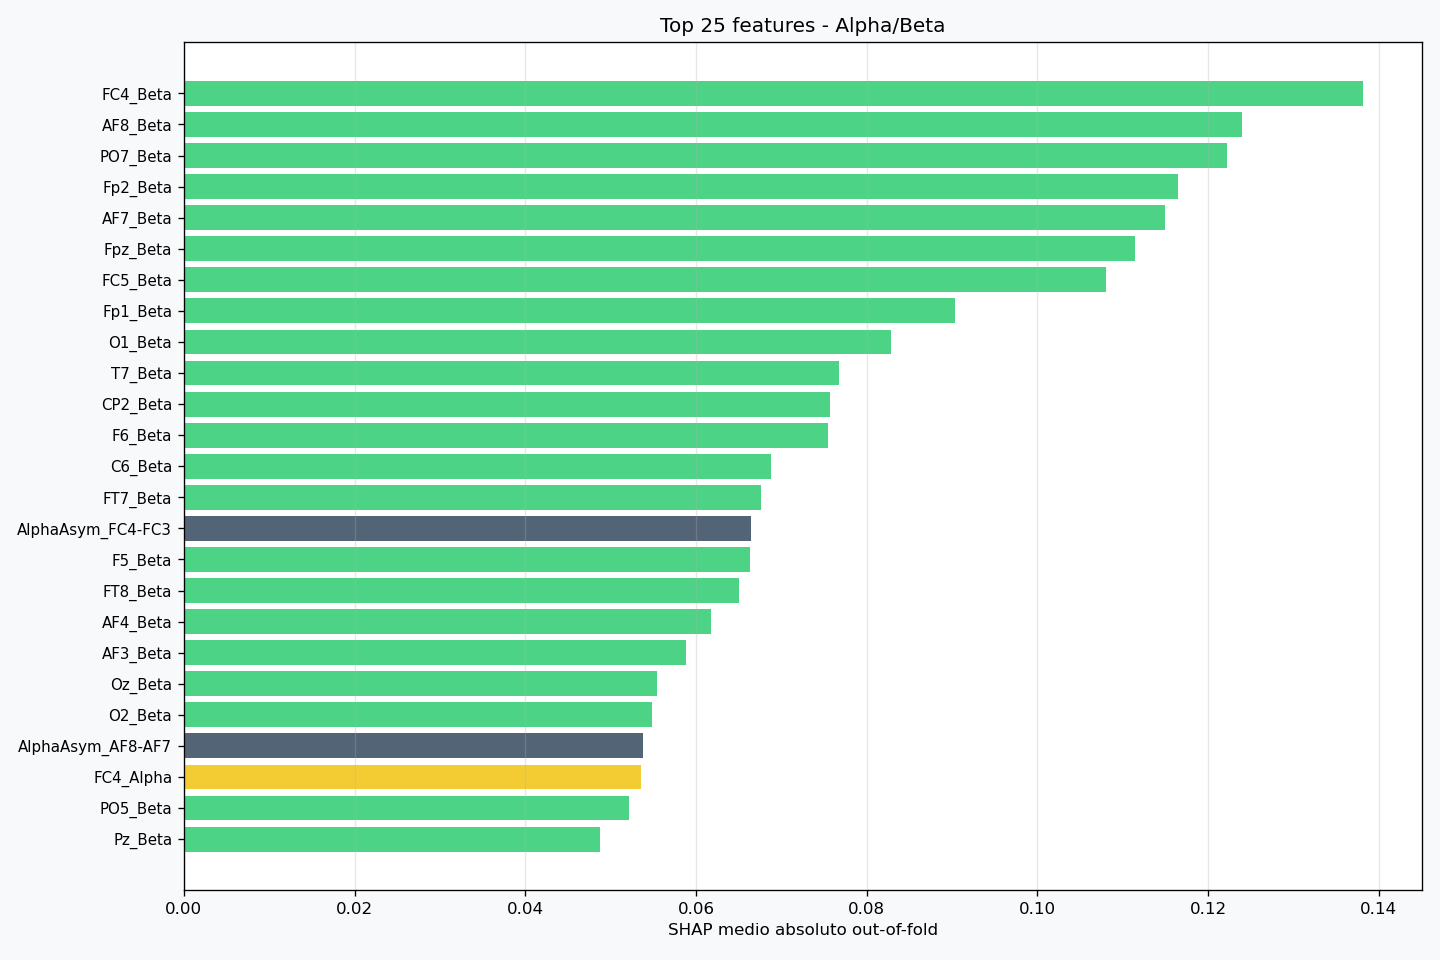
\includegraphics[width=0.88\textwidth]{figs/explicabilidad/01_top_features_global.png}
    \caption{Características con mayor importancia media absoluta según \ac{SHAP} en el modelo \textit{within-subject}.}
    \label{fig:top_features_global}
\end{figure}

El predominio de Beta indica que el modelo da más peso a variaciones relacionadas con actividad rápida dentro del rango seleccionado. En una tarea de escucha pasiva, esto puede ser compatible con diferencias en procesamiento activo, atención o implicación ante el estímulo. La presencia de canales temporales y temporo-parietales resulta coherente con el carácter auditivo y lingüístico de la tarea, mientras que los canales frontales pueden relacionarse con procesos de control, atención y participación cognitiva. Las asimetrías Alpha aparecen, pero con menor peso global que las variables Beta; aun así, su presencia es relevante porque la asimetría Alpha se ha utilizado de forma habitual en estudios de emoción con \ac{EEG} \cite{smith2017frontal}.

\subsection{Importancia por bandas}

La Figura~\ref{fig:band_importance_class} resume la importancia relativa de Alpha y Beta para cada condición emocional. En las tres clases, Beta concentra la mayor parte de la contribución: 76,7\% en \texttt{JOY}, 74,9\% en \texttt{NEUTRO} y 72,7\% en \texttt{SAD}. Alpha mantiene una aportación menor, aunque no desaparece, con valores entre el 23\% y el 27\%.

\begin{figure}[H]
    \centering
    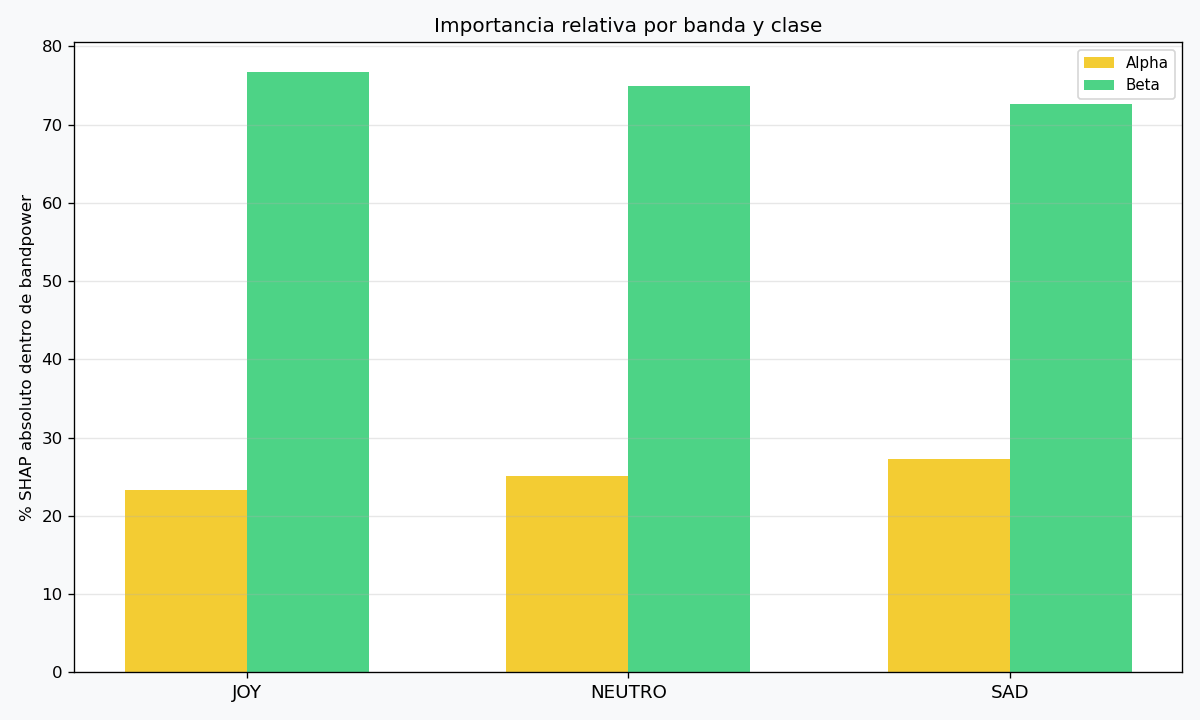
\includegraphics[width=0.78\textwidth]{figs/explicabilidad/02_band_importance_by_class.png}
    \caption{Importancia relativa de las bandas Alpha y Beta por condición emocional.}
    \label{fig:band_importance_class}
\end{figure}

Esta distribución refuerza la lectura anterior: el modelo se apoya principalmente en Beta, pero conserva información complementaria en Alpha. Esto es importante porque evita una interpretación basada en una única banda. Alpha puede seguir aportando diferencias de reposo, lateralización o asimetría, mientras que Beta parece recoger mejor las variaciones asociadas al procesamiento activo de los estímulos.

\subsection{Topomaps globales}

Antes de interpretar los mapas, conviene aclarar qué representa la media global. Estos topomaps no proceden de un único modelo \textit{all-subjects}, sino de agregar las contribuciones \ac{SHAP} calculadas en el análisis \textit{within-subject}. Es decir, primero se obtienen explicaciones dentro de cada participante y después se promedian las contribuciones asociadas a los mismos canales y bandas. Como todos los registros comparten el mismo montaje de electrodos, esta media permite resumir tendencias espaciales comunes sin asumir que todos los sujetos tengan exactamente el mismo patrón.

Entrenar un modelo \textit{all-subjects} obliga al clasificador a aprender una frontera de decisión común para todos los participantes, y esa frontera puede quedar afectada por la variabilidad intersujeto, un problema habitual en \ac{EEG} \cite{rajpoot2022subject}. En cambio, promediar topomaps es una operación descriptiva posterior: no sirve para tomar decisiones sobre nuevas épocas, sino para observar qué zonas aparecen con mayor frecuencia en las explicaciones individuales. Por tanto, la media global ayuda a visualizar patrones compartidos, mientras que los mapas por sujeto siguen siendo necesarios para comprobar cuánto cambia esa distribución entre participantes.

Los mapas topográficos firmados permiten observar dónde contribuyen más las características hacia cada clase. En estas figuras, los colores rojizos representan contribuciones positivas hacia la emoción indicada y los azulados contribuciones negativas. Al estar basados en \ac{SHAP}, no muestran potencia cerebral absoluta, sino cómo las características de cada zona empujan la decisión del modelo hacia una clase concreta.

\begin{figure}[H]
    \centering
    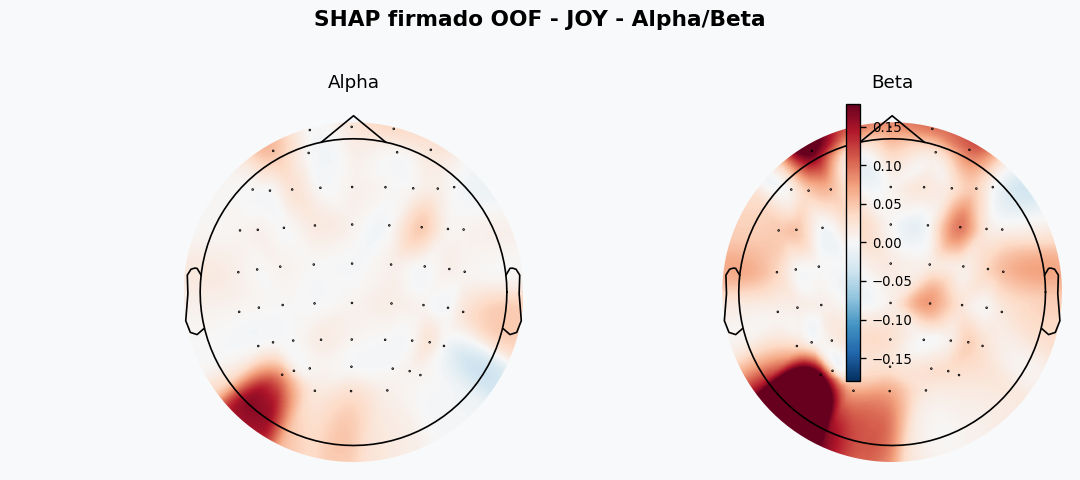
\includegraphics[width=0.82\textwidth]{figs/explicabilidad/04_topomap_signed_JOY.png}
    \caption{Topomap firmado de \ac{SHAP} para la clase \texttt{JOY}.}
    \label{fig:topomap_signed_joy}
\end{figure}

En la Figura~\ref{fig:topomap_signed_joy}, \texttt{JOY} muestra contribuciones positivas destacadas en Beta sobre zonas frontales y posteriores. Esta distribución es compatible con una mayor implicación del participante durante los estímulos de alegría: aparecen regiones frontales, relacionadas de forma general con atención y control cognitivo, junto con zonas temporales/posteriores implicadas en el procesamiento auditivo y del contenido escuchado. No se debe afirmar que estas áreas estén ``activadas'' en sentido clínico, pero sí que el modelo encuentra información discriminativa en esa distribución espacial.

\begin{figure}[H]
    \centering
    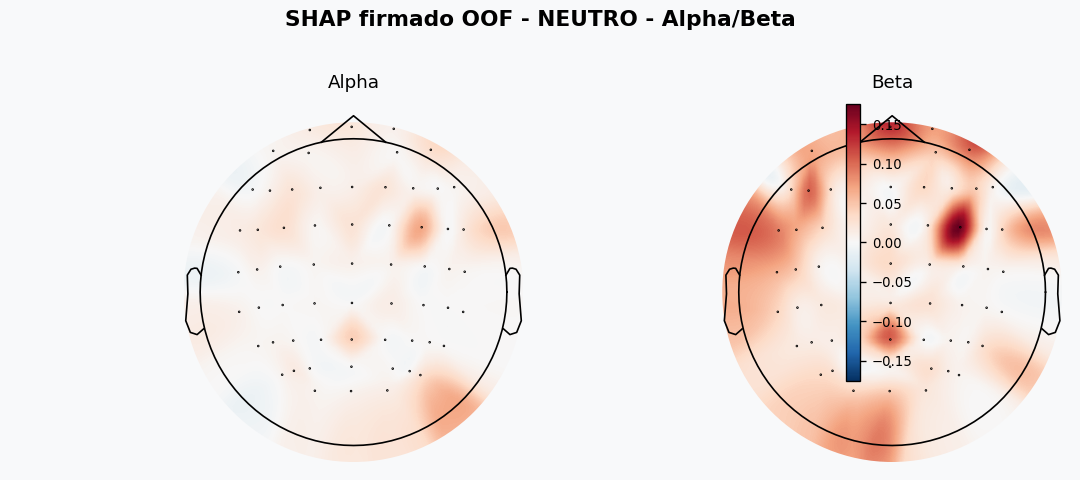
\includegraphics[width=0.82\textwidth]{figs/explicabilidad/04_topomap_signed_NEUTRO.png}
    \caption{Topomap firmado de \ac{SHAP} para la clase \texttt{NEUTRO}.}
    \label{fig:topomap_signed_neutro}
\end{figure}

La Figura~\ref{fig:topomap_signed_neutro} presenta una distribución más localizada. Aunque Beta sigue siendo la banda dominante, la contribución aparece menos extendida que en \texttt{JOY}. Esto encaja con la idea de que la condición neutra actúa como una referencia de menor carga emocional: el modelo no necesita una respuesta espacial tan amplia, sino patrones concretos que diferencian estas épocas de las otras dos condiciones.

\begin{figure}[H]
    \centering
    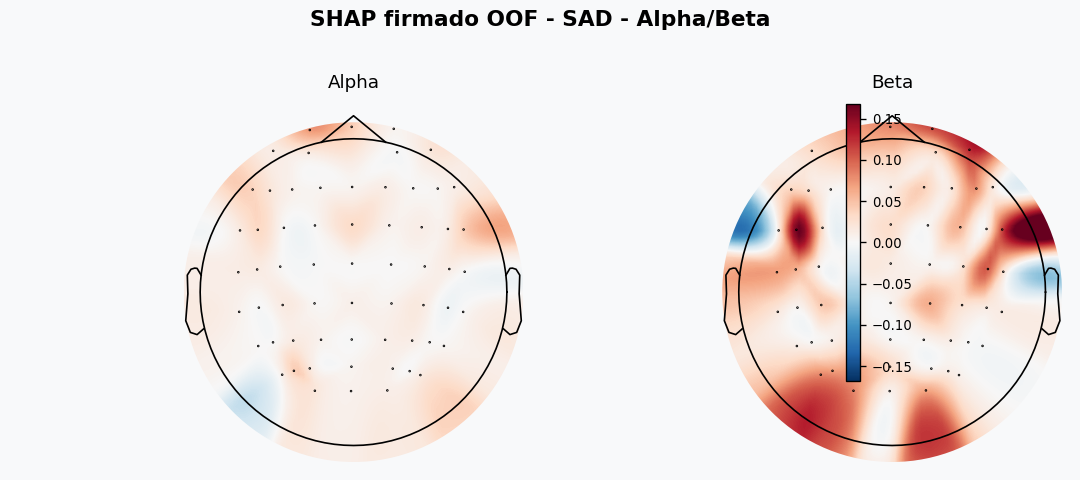
\includegraphics[width=0.82\textwidth]{figs/explicabilidad/04_topomap_signed_SAD.png}
    \caption{Topomap firmado de \ac{SHAP} para la clase \texttt{SAD}.}
    \label{fig:topomap_signed_sad}
\end{figure}

En la Figura~\ref{fig:topomap_signed_sad}, \texttt{SAD} mantiene contribuciones relevantes en Beta, pero con una distribución distinta a la de \texttt{JOY}. Se aprecian zonas temporales y posteriores, junto con un patrón frontal menos homogéneo. Esta diferencia espacial ayuda a explicar por qué el modelo distingue bien las tres clases dentro de sujeto: no solo cambia la magnitud de las contribuciones, sino también la localización relativa de las características que empujan la predicción.

\subsection{Diferencias entre sujetos}

La explicabilidad también confirma que los patrones no son idénticos entre participantes. Las Figuras~\ref{fig:topomap_subject_547_552} muestran los topomaps firmados de los sujetos 211-000547 y 211-000552, dos participantes que ya se habían utilizado como ejemplo en el análisis de separabilidad. Ambos obtienen buen rendimiento en el modelo \textit{within-subject}, pero la distribución espacial de las contribuciones no es igual.

\begin{figure}[H]
    \centering
    \begin{minipage}{0.48\textwidth}
        \centering
        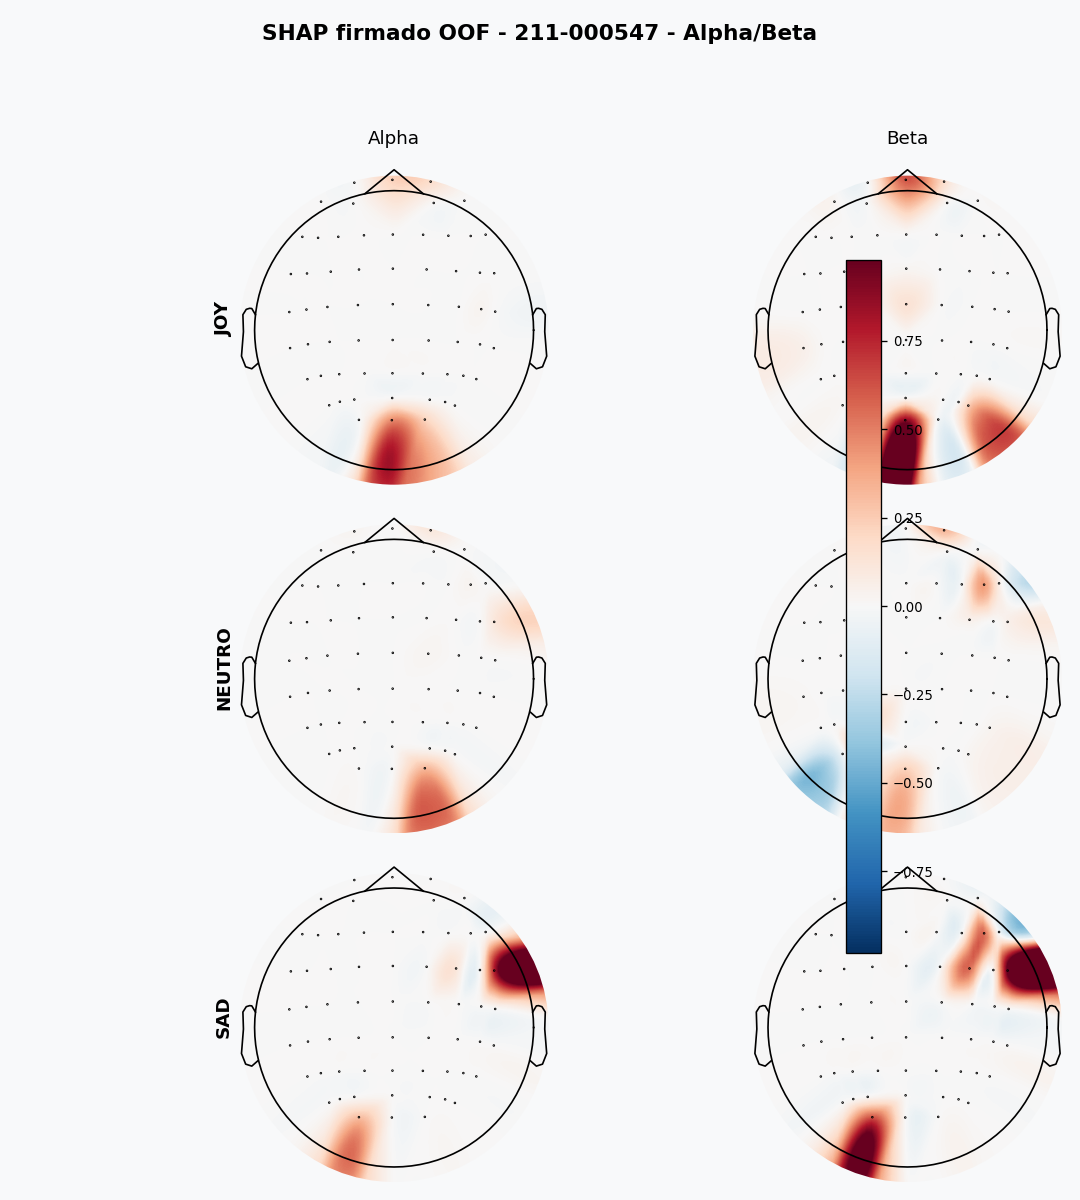
\includegraphics[width=\textwidth]{figs/explicabilidad/topomap_signed_211-000547.png}

        \small Sujeto 211-000547
    \end{minipage}
    \hfill
    \begin{minipage}{0.48\textwidth}
        \centering
        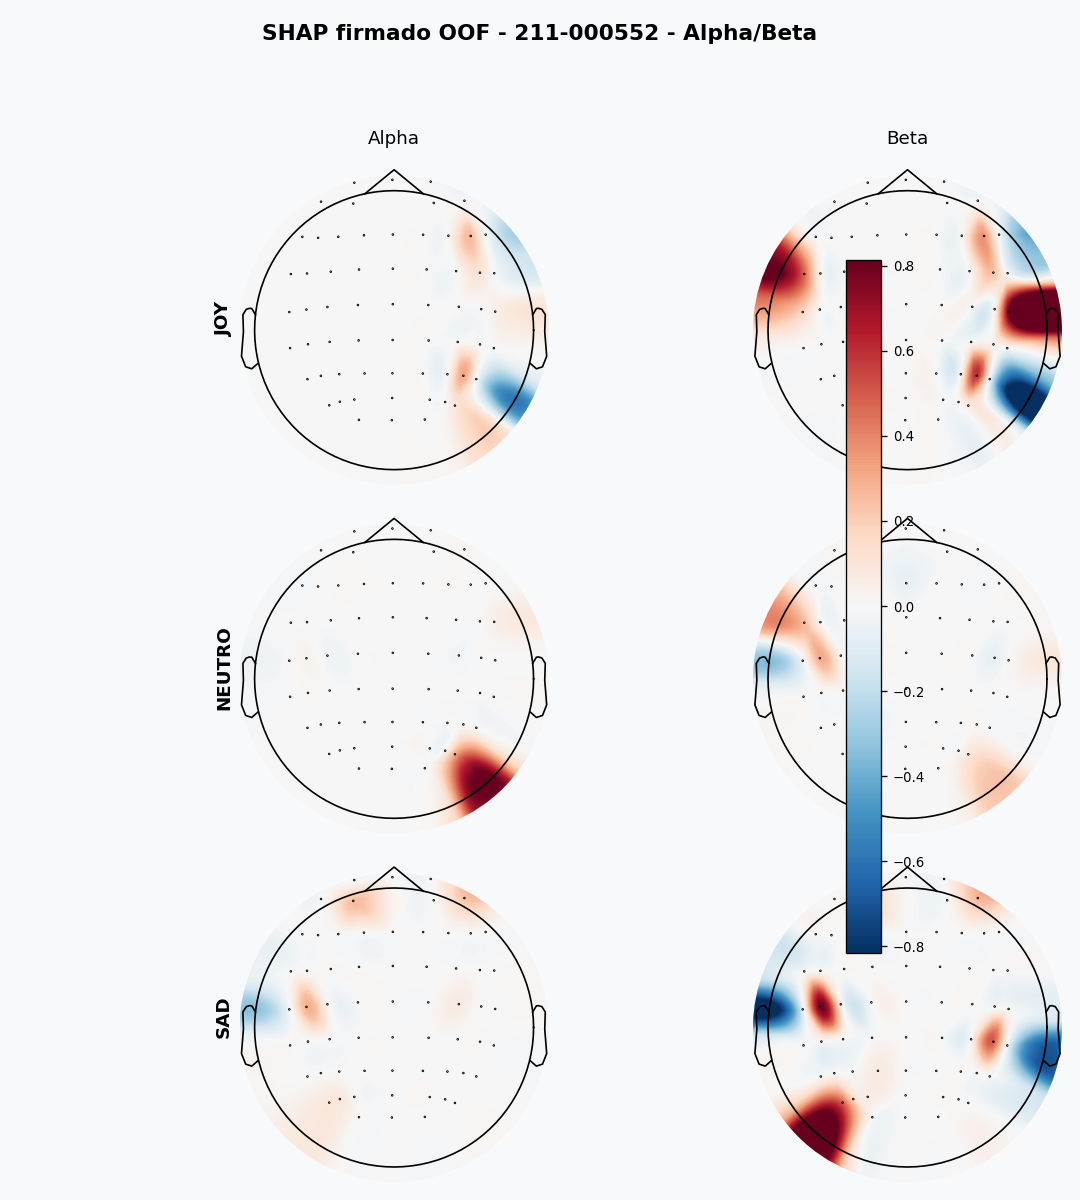
\includegraphics[width=\textwidth]{figs/explicabilidad/topomap_signed_211-000552.png}

        \small Sujeto 211-000552
    \end{minipage}
    \caption{Topomaps firmados por sujeto para dos participantes representativos.}
    \label{fig:topomap_subject_547_552}
\end{figure}

En el sujeto 211-000547, las contribuciones aparecen más concentradas en zonas posteriores y laterales, con patrones muy marcados para \texttt{JOY} y \texttt{SAD}. En el sujeto 211-000552, en cambio, se observa una distribución más lateralizada y con diferencias más visibles entre Alpha y Beta. Esta variabilidad no contradice el buen rendimiento del modelo; al contrario, explica por qué el enfoque \textit{within-subject} funciona mejor que el modelo global. Cada participante puede presentar una organización espacial propia, y el clasificador aprovecha esas regularidades internas sin obligarlas a coincidir exactamente con las de otros sujetos.

\subsection{Agrupación por clusters}

Para interpretar los mapas sin depender de electrodos aislados, las características se agruparon en clusters funcionales de canales. Estos clusters no deben entenderse como regiones anatómicas exactas, sino como agrupaciones prácticas de electrodos próximos o funcionalmente relacionados: temporal izquierdo, temporal derecho, frontal inferior izquierdo, frontal bilateral, centro-parietal izquierdo, parietal medio y occipital.

De forma resumida, los grupos utilizados tienen la siguiente interpretación:

\begin{itemize}
    \item \textbf{Temporal izquierdo}: incluye canales como \texttt{T7}, \texttt{TP7}, \texttt{CP5}, \texttt{CP3}, \texttt{FT7} o \texttt{C5}. Se relaciona con procesamiento auditivo y comprensión del contenido verbal.
    \item \textbf{Temporal derecho}: agrupa canales como \texttt{T8}, \texttt{TP8}, \texttt{CP6} y \texttt{CP4}. Es el homólogo derecho y puede aportar información relacionada con prosodia, entonación y matices emocionales de la escucha.
    \item \textbf{Frontal inferior izquierdo}: incluye \texttt{F7}, \texttt{FC5} y \texttt{F5}. Se considera relevante para procesos activos de lenguaje, como análisis verbal y procesamiento sintáctico.
    \item \textbf{Frontal bilateral}: incluye canales frontales y frontopolares como \texttt{F3}, \texttt{Fz}, \texttt{F4}, \texttt{Fp1} y \texttt{Fp2}. Se interpreta de forma prudente como una zona relacionada con atención, control cognitivo e implicación ante el estímulo.
    \item \textbf{Centro-parietal izquierdo}: agrupa \texttt{C3}, \texttt{CP3} y \texttt{P3}. Puede reflejar integración fonológica o semántica, aunque su interpretación es menos específica que la de los clusters temporales y frontales.
    \item \textbf{Parietal medio}: incluye \texttt{Pz} y \texttt{CPz}. Se utiliza como referencia de integración y atención general, sin asignarle un papel principal en la tarea.
    \item \textbf{Occipital}: incluye \texttt{O1}, \texttt{Oz}, \texttt{O2} y canales próximos. No es el núcleo de una tarea auditiva, pero puede aparecer asociado a atención, visualización mental o diferencias individuales durante la escucha.
\end{itemize}

\begin{figure}[H]
    \centering
    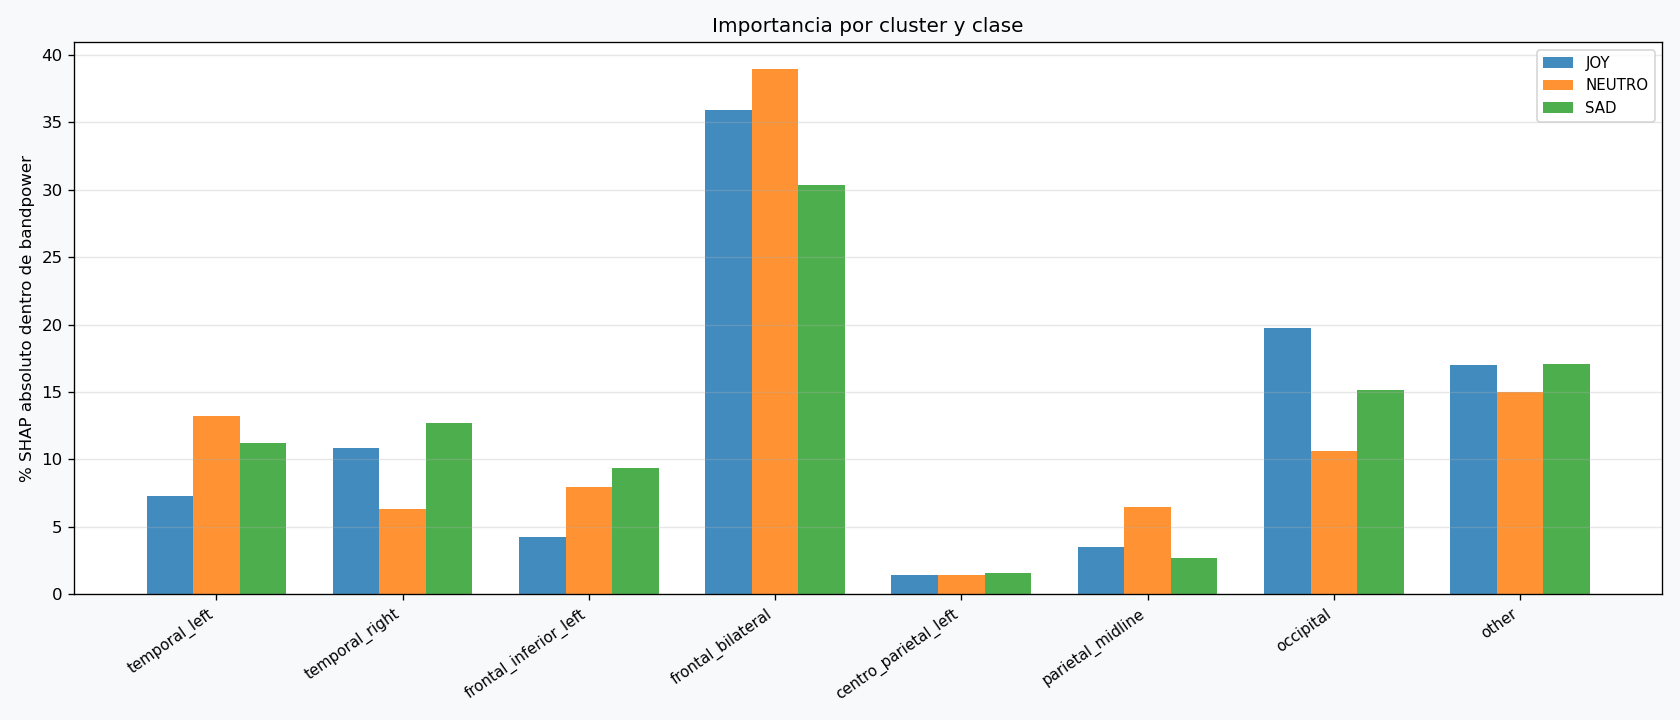
\includegraphics[width=0.88\textwidth]{figs/explicabilidad/05_cluster_importance_by_class.png}
    \caption{Importancia relativa por cluster y condición emocional.}
    \label{fig:cluster_importance_class}
\end{figure}

La Figura~\ref{fig:cluster_importance_class} muestra que el cluster frontal bilateral es el más relevante en las tres condiciones, con mayor peso en \texttt{NEUTRO} y \texttt{JOY} y algo menor en \texttt{SAD}. También aparecen contribuciones importantes en el cluster occipital y en los clusters temporales. La presencia de canales temporales es esperable en una tarea basada en estímulos auditivos, ya que estas zonas participan en el procesamiento de información sonora y lingüística. La contribución frontal puede interpretarse de forma prudente como una señal de participación atencional o procesamiento activo del estímulo.

El cluster occipital no es el núcleo principal de una tarea auditiva, pero su aparición no debe descartarse automáticamente. Puede reflejar diferencias de atención, visualización mental o variabilidad individual durante la escucha. Aun así, se interpreta con cautela, porque los topomaps no permiten afirmar procesos cognitivos complejos como empatía, imaginación o teoría de la mente sin medidas neuropsicológicas adicionales.

\subsection{Resumen de explicabilidad}

El análisis de explicabilidad es coherente con los resultados obtenidos en el entrenamiento. En los modelos \textit{within-subject}, las decisiones se apoyan principalmente en características asociadas a la potencia Beta, con especial presencia en zonas frontales, temporales y posteriores. La potencia Alpha y las asimetrías Alpha también aportan información, aunque con un papel más complementario.

Aun así, las diferencias entre sujetos siguen siendo visibles. Por ello, los resultados no deben interpretarse como la existencia de un patrón universal de \ac{EEG} para cada emoción, sino como la presencia de regularidades individuales que, dentro de cada participante, permiten diferenciar las tres condiciones analizadas.

